%!TEX root = JakubJedryszek-MasterThesis.tex

\cleardoublepage


\chapter{PCA pump prototype implementation and code generation}
\label{pcapumpimpl}

This chapter describes running SPARK Ada programs on BeagleBoard-xM platform (\ref{pcapump:beagleboard}), implementation details of PCA pump prototype (\ref{pcapumpimpl:manual})), code generation from simplified AADL/BLESS models of PCA pump (\ref{pcapumpimpl:codegen}) and overview of not generated parts, which has to be implemented by developer (\ref{pcapumpimpl:codegenimpl}). All programs presented in this section works the same on Intel processor (PC or MacBook) and on BeagleBoard-xM (ARM device).


\section{Running SPARK Ada programs on BeagleBoard-xM}
\label{pcapumpimpl:beagleboard}

To run SPARK Ada program on BeagleBoard-xM, it has to be cross-compiled. As an IDE for SPARK Ada development, GNAT Programming Studio (GPS) is used (see section \ref{background:spark:gps}). To create "Hello, World!" application, new Ada project has been created (choosing Project/New... from the menu). Then main.adb file, with procedure Main printing "Hello, World!" in standard output, was added. The code is presented in listing \ref{listing:HelloWorld}. It is valid Ada 2005 and Ada 2012 code.

\begin{lstlisting}[language=ada, frame=single, gobble=0, caption={"Hello World" in Ada}]
with Ada.Text_IO;

procedure Main
is
begin
    Ada.Text_IO.Put_Line("Hello, World!");    
end Main;
\end{lstlisting} 
\label{listing:HelloWorld}

The main file has to be always specified in project file (\lstinline{.gpr}) in order to compile and link application, which can be runnable. It can be done in Project/Edit Project Properties (figure \ref{figure:editprojectproperties}), tab: Main files (figure \ref{figure:mainfiles}) or directly in project file (\lstinline{.gpr}).

\begin{figure}[ht]%t=top, b=bottom, h=here
    \begin{center}
    	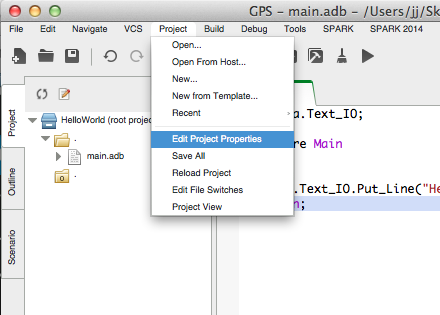
\includegraphics[width=3.2in]{figures/EditProjectProperties.png}
    	\caption{Edit Project Properties}
    \end{center}
    \label{figure:editprojectproperties}
\end{figure}

\begin{figure}[ht]%t=top, b=bottom, h=here
    \begin{center}
    	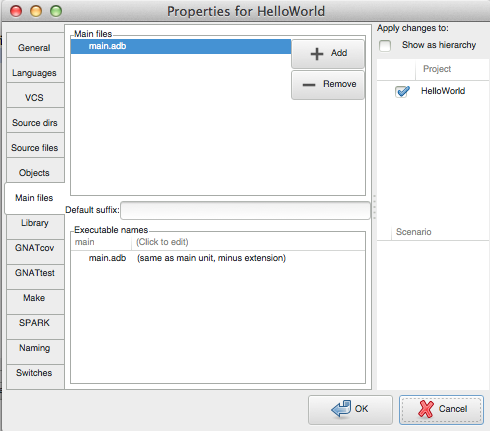
\includegraphics[width=3.2in]{figures/Properties-MainFiles.png}
    	\caption{Project Main files}
    \end{center}
    \label{figure:mainfiles}
\end{figure}

Entire project can be compiled and linked with following command: \lstinline{arm-linux-gnueabi-gnatmake -d -Phelloworld.gpr} (where \lstinline{helloworld.gpr} is GNAT Programming Studio project file). Addditional flags can be specified in command line or directly in project file (manually or through GNAT Programming Studio Interface).

More complex example, which takes advantage of SPARK contracts is presented in section \ref{pcapumpimpl:beagleboard:odometer}.

\subsection{Odometer}
\label{pcapumpimpl:beagleboard:odometer}

Odometer is a simple SPARK Ada program, which implements basic functions of standard Odometer. Listing \ref{listing:Odometer2005} shows Odometer in SPARK 2005. In addition to \lstinline{Odometer}

\singlespacing
\begin{lstlisting}[language=ada, frame=single, gobble=0, caption={SPARK 2005 code: Odometer}]
	package Odometer
	--# own
	--# Trip,        -- number of meters so far on this trip (can be reset to 0).
	--# Total        -- total meters traveled of vehicle since the last factory-reset.
	--#   : Natural; -- has range 0 .. Integer'Last.
	--# initializes Trip,
	--#             Total;
	is
	    procedure Zero_Trip; -- sets Trip to 0 and clears all saved Trip marks.
	    --# global out Trip;
	    --# derives Trip from ;
	    --# post Trip = 0;
	    
	    function Read_Trip return Natural; -- returns value of Trip.
	    --# global in Trip;
	    --# return Trip;
	    
	    function Read_Total return Natural; -- returns value of Total
	    --# global in Total;
	    --# return Total;
	    
	    procedure Inc; -- increments each of Trip and Total by 1.
	    --# global in out Trip, Total;
	    --# derives Trip from Trip & Total from Total;
	    --# pre Trip < Integer'Last and Total < Integer'Last;
	    --# post Trip = Trip~ + 1 and Total = Total~ + 1;	    
	end Odometer;

	package body Odometer is
	    Trip : Natural := 0;
	    Total : Natural := 0;
	    
	    procedure Zero_Trip is
	    begin
	        Trip := 0;
	    end Zero_Trip;
	    
	    function Read_Trip return Natural is
	    begin
	        return Trip;
	    end Read_Trip;
	    
	    function Read_Total return Natural is
	    begin
	        return Total;
	    end Read_Total;
	    
	    procedure Inc is
	    begin
	        Trip := Trip + 1;
	        Total := Total + 1;
	    end Inc;	    
	end Odometer;
\end{lstlisting} 
\label{listing:Odometer2005}
\doublespacing

There are 4 subprograms (2 procedures and 2 functions), which are globally available (through other packages and program units):
\begin{itemize}
    \item Zero\_Trip procedure - reset Odometer to 0
    \item Read\_Trip function - returns current distance
    \item Read\_Total function - returns total distance traveled
    \item Inc procedure - increment total and current distance by 1
\end{itemize}

Given program contains code contracts. Tough it does not matter in compilation phase, it shows that SPARK verification tools can be used for given example. 

Annotation \lstinline{global} means that subprogram uses some global variable. Postfix in, out or in out means that particular variable is read, write or read and write respectively. Annotation \lstinline{derives} says that some variable value depends on other variables. E.g. in procedure \lstinline{Inc} variable \lstinline{Trip} is dependent on its current value (before procedure call). Annotations \lstinline{pre} and \lstinline{post} define pre- and postconditions of procedure. We can see, that in \lstinline{Zero_Trip} procedure postcondition requires that variable \lstinline{Trip} is equal to 0. In procedure \lstinline{Inc}, postconditions requires that variables \lstinline{Trip} and \lstinline{Total} are incremented by 1 ('\lstinline{~}' is the value of variable before procedure call). Annotation \lstinline{own} expose private variables for use in public methods specification. Annotation \lstinline{initializes} ensures that given variables are initializes. 

In order to test \lstinline{Odometer} package in runtime, the \lstinline{Main} procedure has been created. It is presented in listing \ref{listing:main}.


\singlespacing
\begin{lstlisting}[language=ada, frame=single, gobble=0, caption={Main procedure for \lstinline{Odometer} package}]
	with Ada.Text_IO;
	with Odometer;
	procedure Main
	is
	begin
	    Ada.Text_IO.Put_Line("Trip:  " & Natural'Image(Odometer.Read_Trip));
	    Ada.Text_IO.Put_Line("Total: " &  Natural'Image(Odometer.Read_Total));

	    Odometer.Inc;

	    Ada.Text_IO.Put_Line("Trip:  " & Natural'Image(Odometer.Read_Trip));
	    Ada.Text_IO.Put_Line("Total: " &  Natural'Image(Odometer.Read_Total));

	    Odometer.Zero_Trip;

	    Ada.Text_IO.Put_Line("Trip:  " & Natural'Image(Odometer.Read_Trip));
	    Ada.Text_IO.Put_Line("Total: " &  Natural'Image(Odometer.Read_Total));

	    Odometer.Inc;

	    Ada.Text_IO.Put_Line("Trip:  " & Natural'Image(Odometer.Read_Trip));
	    Ada.Text_IO.Put_Line("Total: " &  Natural'Image(Odometer.Read_Total));
	end Main;
\end{lstlisting} 
\label{listing:main}
\doublespacing

Odometer in SPARK 2005 works fine on BeagleBoard-xM. In order to test SPARK 2014 program, SPARK 2005 annotations has been converted into Ada 2012 contracts. Listing \ref{listing:Odometer2014} presents Odometer in SPARK 2014.

\singlespacing
\begin{lstlisting}[language=ada2012, frame=single, gobble=0, caption={SPARK 2014 code: Odometer}, label={listing:Odometer2014}]
	package Odometer
	with Abstract_State => (Trip_State, Total_State)
	is
	   function Trip_State return Integer
	     with Convention => Ghost,
	     Global => (Input => Trip_State);

	   function Total_State return Integer
	     with Convention => Ghost,
	     Global => (Input => Total_State);

	   procedure Zero_Trip -- sets Trip to 0
	     with Global => (Output => (Trip_State)),
	     Depends => (Trip_State => null),
	     Post => Trip_State = 0;

	   function Read_Trip return Natural -- returns value of Trip.
	     with Global => (Input => Trip_State),
	     Post => Read_Trip'Result = Trip_State;

	   function Read_Total return Natural -- returns value of Total
	     with Global => (Input => Total_State),
	     Post => Read_Total'Result = Total_State;

	   procedure Inc -- increments each of Trip and Total by 1.
	     with Global => (In_Out => (Trip_State, Total_State)),
	     Depends => (Trip_State => Trip_State, Total_State => Total_State),
	     Pre => Trip_State < Integer'Last and Total_State < Integer'Last,
	     Post => Trip_State = Trip_State'Old + 1 and Total_State = Total_State'Old + 1;
	end Odometer;

	package body Odometer
	with
	  Refined_State => (Trip_State => (Trip),
	                    Total_State => (Total))
	is
	   Trip : Natural;
	   Total : Natural;

	   function Trip_State return Integer
	     with Refined_Global => (Input => Trip)
	   is
	   begin
	      return Trip;
	   end Trip_State;

	   function Total_State return Integer
	     with Refined_Global => (Input => Total)
	   is
	   begin
	      return Total;
	   end Total_State;

	   procedure Zero_Trip
	     with Refined_Global => (Output => Trip),
	     Refined_Depends => (Trip => null)
	   is
	   begin
	      Trip := 0;
	   end Zero_Trip;

	   function Read_Trip return Natural
	     with Refined_Global => (Input => Trip)
	   is
	   begin
	      return Trip;
	    end Read_Trip;

	   function Read_Total return Natural
	     with Refined_Global => (Input => Total)
	   is
	   begin
	      return Total;
	   end Read_Total;

	   procedure Inc
	     with Refined_Global => (In_Out => (Trip, Total)),
	     Refined_Depends => (Trip => Trip, Total => Total)
	   is
	   begin
	      Trip := Trip + 1;
	      Total := Total + 1;
	   end Inc;
	end Odometer;
\end{lstlisting}
\doublespacing

Odometer example was created to check possible limitations or issues related to different platform and processor (ARM). No limitations were found.


\subsection{Multitasking applications}
\label{pcapumpimpl:beagleboard:multitasking}

In Ada World, concurrency is referred as tasking and the task is the same construct as the thread in other programming languages. In section \ref{pcapumpimpl:beagleboard:odometer}, single-tasking application was tested. This section presents simple Ada multitasking application and multitasking version of Odometer in SPARK 2005 from section \ref{pcapumpimpl:beagleboard:odometer}. Both applications compiles correctly and works as expected on BeagleBoard-xM platform.

\subsubsection{Ada multitasking application}

Listing \ref{listing:HelloTasking} presents a simple multitasking application printing numbers in different time intervals, in Ada 2005. It is also valid code for Ada 2012. There are 3 tasks:
\begin{itemize}
    \item Main task
    \item S (type: \lstinline{Seconds}) - simple counter printing numbers form 1 to 10 in every second
    \item T (type: \lstinline{Tenth_Seconds}) - simple counter printing numbers from 0.1 to 10 in every 0.1 second
\end{itemize}

\begin{lstlisting}[language=ada, frame=single, gobble=0, caption={Simple multitask application in Ada}]
	with Ada.Text_IO;
	use Ada.Text_IO;
	with Ada.Float_Text_IO;

	procedure Main is
	    task type Seconds is
	    end Seconds;

	    task type Tenth_Seconds is
	    end Tenth_Seconds;

	    S : Seconds;
	    T : Tenth_Seconds;

	    task body Seconds is
	    begin
	        for I in 1..10 loop
	            delay Standard.Duration(1);
	            Put_Line(Integer'Image(I));
	        end loop;
	    end Seconds;

	    task body Tenth_Seconds is
	    begin
	        for I in 1..100 loop            
	            delay 0.1;            
	            Ada.Float_Text_IO.Put(Float(I)/Float(10), AFT=>2, EXP=>0);
	            Put_Line("");
	        end loop;
	    end Tenth_Seconds;
	begin
	    Put_Line("Started");
	end Main;
\end{lstlisting} 
\label{listing:HelloTasking}

The program works as expected on BleagleBoard-xM. This is not valid SPARK program though. As mentioned in section \ref{background:spark:ravenscar}, tasks can be declared only in packages. Not in subprograms or in other tasks. \cite{Barnes:Book} 

\subsubsection{SPARK Ada multitasking application}

As mentioned in section \ref{background:spark:ravenscar}, in SPARK 2005 multitasking is possible with Ravenscar Profile. Default profile - sequential -  does not enable tasking. In other words, SPARK tools cannot analyze and reason about programs if Ravenscar profile flag is not provided. In SPARK 2014 - for now tasking is not possible. It's part of SPARK 2014 road map to include support for tasking in the future. Thus, only SPARK 2005 application was tested.

Tested, multitasking application is extended version of Odometer presented in listing \ref{listing:Odometer2005}. It has additional variable \lstinline{Speed}, procedure \lstinline{Set_Speed} and new task: \lstinline{Drive}. Thus, in total it has two tasks:
\begin{itemize}
    \item Main
    \item Drive
\end{itemize}

The \lstinline{Drive} task increase \lstinline{Total} and \lstinline{Trip} variables by \lstinline{Speed} (m/s) in every second. Extended Odometer is presented in listing \ref{listing:Odometer2005Tasking}. 

\begin{lstlisting}[language=ada, frame=single, gobble=0, caption={Multitasking Odometer}]
	--# inherit Ada.Real_Time;
	package Odometer
	--# own Trip : Distance;
	--#     Total : Distance;
	--#     Speed : Meters_Per_Second;
	--#     task d : Drive;
	--# initializes Trip, 
	--#             Total,
	--#             Speed;
	is
	    type Distance is range Natural'First .. Natural'Last;
	    pragma Atomic (Distance);
	    
	    type Meters_Per_Second is range Natural'First .. Natural'Last;
	    pragma Atomic(Meters_Per_Second);
	    
	    procedure Zero_Trip; -- sets Trip to 0 and clears all saved Trip marks.
	    --# global out Trip;
	    --# derives Trip from ;
	    --# post Trip = 0;
	    
	    function Read_Trip return Distance; -- returns value of Trip.
	    --# global in Trip;
	    --# return Trip;
	    
	    function Read_Total return Distance; -- returns value of Total
	    --# global in Total;
	    --# return Total;
	    
	    procedure Inc; -- increments each of Trip and Total by 1.
	    --# global in out Trip, Total;
	    --# derives Trip from Trip & Total from Total;
	    --# pre Trip < Distance'Last and Total < Distance'Last;
	    --# post Trip = Trip~ + 1 and Total = Total~ + 1;

	    procedure Set_Speed(New_Speed : Meters_Per_Second);
	    --# global out Speed;
	    --# derives Speed from New_Speed;
	    --# post Speed = New_Speed;                             
	private    	    
	    task type Drive
	    --# global in     Speed;
	    --#        in out Trip;
	    --#        in out Total;
	    --#        in     Ada.Real_Time.ClockTime;
	    is
	        pragma Priority(10);
	    end Drive;	    
	end Odometer;

	with Ada.Real_Time;
	use type Ada.Real_Time.Time;
	package body Odometer is
	    Trip : Distance := 0;
	    Total : Distance := 0;
	    Speed : Meters_Per_Second := 0;
	    d : Drive;
	    
	    procedure Zero_Trip is
	    begin
	        Trip := 0;
	    end Zero_Trip;
	    
	    function Read_Trip return Distance is
	    begin
	        return Trip;
	    end Read_Trip;
	    
	    function Read_Total return Distance is
	    begin
	        return Total;
	    end Read_Total;
	    
	    procedure Inc is
	    begin
	        Trip := Trip + 1;
	        Total := Total + 1;
	    end Inc;
	    
	    procedure Set_Speed(New_Speed : Meters_Per_Second)
	    is
	    begin
	        Speed := New_Speed;
	    end Set_Speed;    
	    
	    task body Drive
	    is
	        Release_Time : Ada.Real_Time.Time;
	        Period : constant Integer := 1000; -- update in every second
	    begin
	        loop
	            Release_Time := Ada.Real_Time.Clock + Ada.Real_Time.Milliseconds(Period);
	            delay until Release_Time;
	            -- each time round, increase Trip and Total
	            for I in Meters_Per_Second range 0 .. Speed loop
	                Inc;
	            end loop;            
	        end loop;
	    end Drive;
	    	end Odometer;
\end{lstlisting} 
\label{listing:Odometer2005Tasking}

There are two ways to access protected variable in task body:
\begin{itemize}
    \item It has to be protected object
    \item It has to be atomic type
\end{itemize}

Protected variables may not be used in proof contexts. Thus, if we try to use protected variable in proofs (pre- or postcondition), then we get semantic error: \lstinline{Trip is a protected own variable}. To preserve pre- and postconditions from original Odometer, atomic types (\lstinline{Distance} and \lstinline{Meters_Per_Second}) has been used. The capability to specify pre- and postconditions has been preserved, but now application is not thread safe.


\subsection{Controlling PCA pump motor}
\label{pcapumpimpl:beagleboard:pcapumpmotor}

PCA pump prototype created as part of this thesis interacts with external device (pump motor) through GPIO ports. 

// pca motor


Expansion port 14(PWM) and 28(GND?)
GPIO158
memory mapped ports
Java Program to Run the pump for 10 seconds
Include source of simple program?


\section{Implementation based on Requirements Document and AADL models}
\label{pcapumpimpl:manual}

First step was to create mock (based on doc, aadl models and implemented PCA Pump).

In this thesis, only the operation module is implemented. Req doc don't specified all implementation details, like how basal rate should be infused.

The first step, was to check if implementation of PCA Pump specified in Requirements Document is possible. Especially whether it will work on BeagleBoard-xM device. To do that, simple version of PCA Pump based on Requirements Document was created. Only two AADL threads are implemented: \lstinline{Rate_Controler} and \lstinline{Max_Drug_Per_Hour_Watcher} in stripped version.

Pump internal implementation based on \cite{CADD-PrizmAmbulatoryInfusionPump:Online}.
- basal dose deliver in increments - easier to track delivered amount (page 14)

The pump has three tasks in total:
\begin{itemize}
    \item main task (requesting boluses, displaying volume infused etc.)
    \item rate controller - to control the speed of infusion rate
    \item max drug per hour watcher - to control overinfusion
\end{itemize}

The main PCA Pump Package can be verified using SPARK tools. The Pump engine (motor) is separated entity. It has an interface allowing request infusion of 0.1 ml of drug.

PCA Pump prototype was developed based on Requirements Documentation created by Brian Larson, John Hatcliff and Partice Chalin \cite{PcaReq}.

In real-world applications, the embedded critical components are written in SPARK while the non-critical components are written in Ada. Components written in Ada should be hidden for SPARK Examiner with \lstinline{--# hide} annotation or being separated entities on which SPARK tools are not run. PCA motor is separated entity.

//summary
The biggest challenge during PCA Pump development was the SPARK limitations. There are many common libraries, which cannot be verified by SPARK tools. Thus it required to isolate some functionalities or implement them in different way. An example might be reading and writing numbers to standard input.



\section{Code generation from AADL/BLESS models}
\label{pcapumpimpl:codegen}

PCA Pump prototype was mocked using translations schemas from chapter \ref{codegen}.

The original models were simplified and truncated for the purpose of this thesis. Finally only \lstinline{PCA_Operation} module with 3 threads (\lstinline{Max_Drug_Per_Hour_Watcher}, \lstinline{Rate_Controller}, \lstinline{Patient_Bolus_Checker}), types definitions (\lstinline{Base_Types}, \lstinline{PCA_Types}, \lstinline{ICE_Types}, \lstinline{Bless_Types}) and property set \lstinline{PCA_Properties} were used as the source for code translation.

[code listings of aadl model]


Skeleton code 'generated' from simplified AADL models. Then implemented.

Show generated code.



\section{Implementation for generated code}
\label{pcapumpimpl:codegenimpl}

Mocked code was extended (e.g. to Prescription\_Store Set/Get methods for record fields were added).

Overview of issues solved: 
* Bolus options: FBasal + FPatient or FPatient => implemented: FBasal + FPatient (consistent in doc)
5 modes:
* Stopped: F=0
* KVO: F=0.1
* Basal: F=Fbasal
* Patient: F = Fbasal + Fbolus (for vtbi/Fbolus)
* Clinician: F = Fbalsal + Fbolus (for specified time)

Most common Examiner\cite{Examiner:Online} erroes/warnings:
***        Warning                     :302: This expression may be
***        Semantic Error              :725: Protected function or variable XXX may only appear directly in an assignment or return statement.

Discuss implementation of basal infusion: 0.1 ml pulses timed according to the desired rate. (based on CADD-Prizm page 14). Easier bolus monitoring/calculations. Possibility to separate pulse from engine logic. Just array with time stamps(?) or array with size = (60 * 60 /min\_possible\_time\_between\_activations) and set 1 if activation occured. In every second, update array: array[i]=array[i+1]. Array is protected object, so bolus thread cannot access it in the same time, when update thread.
Another option: constant speed of engine and speed-up on boluses. Harder bolus monitoring/calculations?


Internal calculations are in micro liters 1 micro liters ($\mu$l) = 0.001 ml thus 1 ml = 1000$\mu$l.


